\documentclass[10pt,a4paper]{article}

% Encoding & language
\usepackage[utf8]{inputenc}
\usepackage[spanish]{babel}

% Font

% Page layout - tighter to fit 10 pages
\usepackage[a4paper,
  top=2.15cm, bottom=0.7cm,
  left=1.9cm, right=1.9cm,
  headheight=14pt]{geometry}

% Colors
\usepackage[table,dvipsnames]{xcolor}
\definecolor{ink}{HTML}{1a1a1a}
\definecolor{accent}{HTML}{1a3a5c}
\definecolor{rulecol}{HTML}{c8d0da}
\definecolor{rowodd}{HTML}{f0f4f8}
\definecolor{roweven}{HTML}{e4ebf2}
\definecolor{calloutbg}{HTML}{eef2f7}
\definecolor{coverbg}{HTML}{0f2540}
\definecolor{coveraccent}{HTML}{4a90d9}
\definecolor{mutedgray}{HTML}{6b7280}

% Graphics
\usepackage{graphicx}
\usepackage{float}
\usepackage{rotating}
\usepackage[font=small,labelfont=bf,labelsep=period,
            justification=centering]{caption}

% Tables
\usepackage{booktabs}
\usepackage{tabularx}
\usepackage{array}
\usepackage{colortbl}
\graphicspath{{diagrams/}{reports/figures/}}

% Header/footer
\usepackage{fancyhdr}
\pagestyle{fancy}
\fancyhf{}
\renewcommand{\headrulewidth}{0pt}
\fancyhead[L]{\small\color{mutedgray}\itshape
  Plataforma Analítica sobre saleshealth $\cdot$ María Muñoz Nadales}
\fancyhead[R]{\small\color{mutedgray}
  Gestión de Datos --- Data Management}
\fancyfoot[C]{\small\color{mutedgray}\thepage}
\fancypagestyle{plain}{\fancyhf{}\renewcommand{\headrulewidth}{0pt}}

% Section style
\makeatletter
\renewcommand\section{\@startsection{section}{1}{0pt}
  {9pt}{3pt}{\large\bfseries\color{accent}}}
\renewcommand\subsection{\@startsection{subsection}{2}{0pt}
  {6pt}{1pt}{\normalsize\bfseries\color{ink}}}
\makeatother

% Callout box - portable replacement for mdframed
\newsavebox{\calloutbox}
\newenvironment{mdframed}[1][]{
  \par\vspace{3pt}\noindent
  \begin{lrbox}{\calloutbox}
  \begin{minipage}{0.94\textwidth}
}{
  \end{minipage}
  \end{lrbox}
  \begingroup
  \setlength{\fboxsep}{8pt}
  \colorbox{calloutbg}{\usebox{\calloutbox}}
  \endgroup
  \par\vspace{3pt}
}

% Hyperlinks
\usepackage[hidelinks,
  pdftitle={Plataforma Analítica sobre Saleshealth},
  pdfauthor={María Muñoz Nadales}]{hyperref}

% Spacing
\setlength{\parskip}{1.5pt}
\setlength{\parindent}{0pt}
\renewcommand{\baselinestretch}{1.0}

% Table helpers
\newcolumntype{L}[1]{>{\raggedright\arraybackslash}p{#1}}
\newcolumntype{C}[1]{>{\centering\arraybackslash}p{#1}}
\newcolumntype{R}[1]{>{\raggedleft\arraybackslash}p{#1}}
\newcommand{\Th}[1]{\cellcolor{accent}\color{white}\textbf{#1}}
\newcommand{\Ra}{\rowcolor{rowodd}}
\newcommand{\Rb}{\rowcolor{roweven}}
\renewcommand{\toprule}{}
\renewcommand{\midrule}{}
\renewcommand{\bottomrule}{}
\newcommand{\FlowBox}[2]{%
  \colorbox{rowodd}{\begin{minipage}{#1}\centering\scriptsize\textbf{#2}\end{minipage}}}
\newcommand{\MiniBox}[2]{%
  \colorbox{rowodd}{\begin{minipage}{#1}\centering\scriptsize\textbf{\color{accent}#2}\end{minipage}}}

%% ============================================================
\begin{document}
\thispagestyle{empty}

%% ── PORTADA ────────────────────────────────────────────────
\pagecolor{white}\color{ink}
\vspace*{1.55cm}

\begin{center}
{\small\scshape\color{mutedgray}GESTIÓN DE DATOS --- DATA MANAGEMENT}

\vspace{0.22cm}
{\color{rulecol}\hrule height 0.4pt}
\end{center}

\vspace{4.0cm}

{\itshape Proyecto Final}

\vspace{0.35cm}

\begin{minipage}{0.92\textwidth}
\raggedright
{\LARGE\bfseries Plataforma Analítica sobre saleshealth:\par}
\vspace{2pt}
{\LARGE\bfseries DWH, Customer Intelligence y\par}
{\LARGE\bfseries Market Basket\par}
\end{minipage}

\vspace{0.45cm}
\noindent
\begin{minipage}{0.012\textwidth}
  {\color{accent}\rule{2pt}{1.55cm}}
\end{minipage}
\hspace{0.3cm}
\begin{minipage}{0.78\textwidth}
{\raggedright\itshape\color{ink!72}
  Transformación de un sistema transaccional en una plataforma analítica con
  Data Warehouse dimensional,\par
  métricas de cliente, scoring de churn, clustering K-Means, Market Basket
  Analysis y dashboard ejecutivo en Streamlit.\par}
\end{minipage}

\vfill

{\renewcommand{\arraystretch}{1.12}
\begin{tabular}{@{}>{\footnotesize\scshape\color{mutedgray}}l@{\hspace{1.45cm}}>{\small\raggedright\arraybackslash}p{11.0cm}@{}}
  Autora & María Muñoz Nadales \\[5pt]
  Base de datos & saleshealth (PostgreSQL) \\[5pt]
  Tecnologías & PostgreSQL $\cdot$ SQL $\cdot$ Python $\cdot$ Jupyter
      $\cdot$ scikit-learn $\cdot$ Streamlit $\cdot$ Plotly \\[5pt]
  Periodo de datos & Ventas 2020-01-01 $\to$ 2025-12-30
      $\cdot$ Devoluciones hasta 2026-02-07 \\
\end{tabular}}

\vspace{1.1cm}
{\color{rulecol}\hrule height 0.4pt}
\vspace{0.35cm}

{\small\color{mutedgray}
5\,750 clientes $\cdot$ 20\,000 ventas $\cdot$ 42\,555 líneas $\cdot$
9{,}40 M ingresos netos $\cdot$ 3{,}76 M margen neto $\cdot$ 14/14 validaciones OK}

\newpage
\pagecolor{white}\color{ink}

%% ── PÁGINA 1: RESUMEN EJECUTIVO ─────────────────────────────
\section{Resumen ejecutivo}

Este proyecto transforma la base operacional \textbf{saleshealth} en una
plataforma analítica completa. Sobre PostgreSQL se construye un Data Warehouse
dimensional, un proceso ETL reproducible y una capa analítica con métricas de
cliente (CLTV, RFM), scoring de churn, clustering K-Means con PCA, Market
Basket Analysis y un dashboard ejecutivo en Streamlit.

\begin{mdframed}[style=cbox]
\textbf{\color{accent}Hallazgo clave --- calidad de datos}\\[2pt]
El margen supera los 3,76\,M\,EUR, pero 711 líneas dependen de un coste imputado
por una incidencia en el catálogo central (\texttt{product\_id = 29}, «Sensor
temperatura inteligente»). La regla
\texttt{analytic\_unit\_cost = sale\_price * 0{,}60}, trazada con
\texttt{cost\_source} e \texttt{is\_cost\_imputed}, garantiza trazabilidad
total. Corregir el catálogo en origen elimina las 711 líneas imputadas sin
modificar el modelo.
\end{mdframed}

\subsection*{Estructura de la solución}

El proyecto sigue una cadena analítica: base operacional $\to$ DWH $\to$
métricas de cliente $\to$ modelos de segmentación $\to$ dashboard.

\vspace{3pt}
Los objetivos analíticos se agrupan en tres preguntas de negocio: qué clientes
aportan más valor, qué clientes muestran riesgo de abandono y qué productos
pueden recomendarse juntos. La solución evita responderlas con consultas
aisladas: las convierte en artefactos persistentes del DWH, validados y
reutilizables desde notebooks, CSVs y dashboard.

\vspace{3pt}
\begin{tabularx}{\textwidth}{L{2.6cm}L{5.8cm}X}
\toprule
\Th{Capa} & \Th{Componente} & \Th{Resultado} \\
\midrule
\Ra Origen        & 17 tablas operacionales
                  & Base saleshealth (PostgreSQL) \\
\Rb DWH           & 8 dimensiones $\cdot$ 4 hechos
                  & Esquema \texttt{dwh}, grano: línea de venta \\
\Ra ETL           & \texttt{sql/02\_etl.sql} --- transacción atómica
                  & 42\,555 líneas cargadas y validadas \\
\Rb Analítica     & CLTV $\cdot$ RFM $\cdot$ Churn $\cdot$ Clustering $\cdot$ MBA
                  & 5\,750 clientes con score completo \\
\Ra Visualización & Dashboard Streamlit (6 páginas)
                  & Consultable sin conexión a BD \\
\bottomrule
\end{tabularx}

\vspace{5pt}
\textbf{Resultado práctico.} El proyecto no se limita a describir datos
históricos: deja una plataforma operativa para priorizar campañas comerciales,
revisar incidencias de calidad y explotar recomendaciones producto-producto
sin volver a reconstruir las métricas manualmente.

\vspace{6pt}
\begin{center}
\FlowBox{1.75cm}{Origen\\17 tablas}
$\longrightarrow$
\FlowBox{1.75cm}{DWH\\8 dim + 4 hechos}
$\longrightarrow$
\FlowBox{1.75cm}{Métricas\\cliente}
$\longrightarrow$
\FlowBox{1.75cm}{Modelos\\PCA + MBA}
$\longrightarrow$
\FlowBox{1.75cm}{Dashboard\\6 vistas}
\end{center}

%% ── PÁGINA 2: BASE ORIGINAL ─────────────────────────────────
\section{De los datos operacionales al Data Warehouse}

\subsection{La base operacional}

La base \textbf{saleshealth} contiene 17 tablas. Las ventas cubren
2020--2025; las devoluciones llegan hasta febrero 2026. El núcleo
operacional: \texttt{customer $\to$ sale $\to$ sale\_item $\to$ product
$\mid$ store}, con \texttt{sale\_item $\to$ return\_item $\to$
return\_reason} y \texttt{sale\_item $\to$ offer}.

\vspace{3pt}
\begin{tabularx}{\textwidth}{L{2.0cm}L{2.7cm}R{1.3cm}L{2.4cm}L{2.8cm}R{1.2cm}}
\toprule
\Th{Entidad} & \Th{Tabla} & \Th{Filas}
& \Th{Entidad} & \Th{Tabla} & \Th{Filas} \\
\midrule
\Ra Clientes     & \texttt{customer}          & 5\,750
  & Catálogo c.  & \texttt{central\_product}   & 49 \\
\Rb Ventas       & \texttt{sale}              & 20\,000
  & Inv. tienda  & \texttt{inventory}          & 1\,000 \\
\Ra Líneas       & \texttt{sale\_item}        & 42\,555
  & Inv. central & inventario central & 49 \\
\Rb Productos    & \texttt{product}           & 50
  & Marcas/Cat.  & \texttt{brand/category}     & 29/6 \\
\Ra Tiendas      & \texttt{store}             & 20
  & Zonas geog.  & \texttt{city\_zone}         & 42 \\
\Rb Devol.       & \texttt{return\_item}      & 2\,330
  & Almacén      & \texttt{warehouse}          & 1 \\
\Ra Mot. dev.    & \texttt{return\_reason}    & 6
  & Ub. almacén  & ubicaciones & 40 \\
\Rb Ofertas      & ofertas / productos & 1/6
  & & & \\
\bottomrule
\end{tabularx}

\vspace{4pt}
La separación entre ventas, devoluciones, catálogo, tienda e inventario permite
mantener la lógica transaccional original, pero el análisis exige un modelo más
estable. Por eso el diseño dimensional no copia la base origen: selecciona las
entidades relevantes, resuelve relaciones implícitas y conserva trazabilidad
entre claves naturales y claves analíticas.

\newpage
\vspace{6pt}
El análisis de relaciones implícitas reveló cuatro decisiones de modelado:

\vspace{3pt}
\begin{tabularx}{\textwidth}{L{2.1cm}L{5.6cm}X}
\toprule
\Th{Área} & \Th{Hallazgo} & \Th{Decisión en el DWH} \\
\midrule
\Ra Tiendas      & \texttt{postal\_code} cruza con \texttt{city\_zone}
                 & \texttt{dim\_store} enriquecida con distrito y área \\
\Rb Ofertas      & Líneas sin \texttt{offer\_id}
                 & Registro técnico «Sin oferta» \\
\Ra Devoluciones & Motivo no informado
                 & Registro técnico «Sin motivo» \\
\Rb Catálogo     & Producto 29 sin coste
                 & Coste analítico imputado al 60\% del precio,
                   trazado con flag de imputación \\
\bottomrule
\end{tabularx}

\begin{figure}[H]
\centering
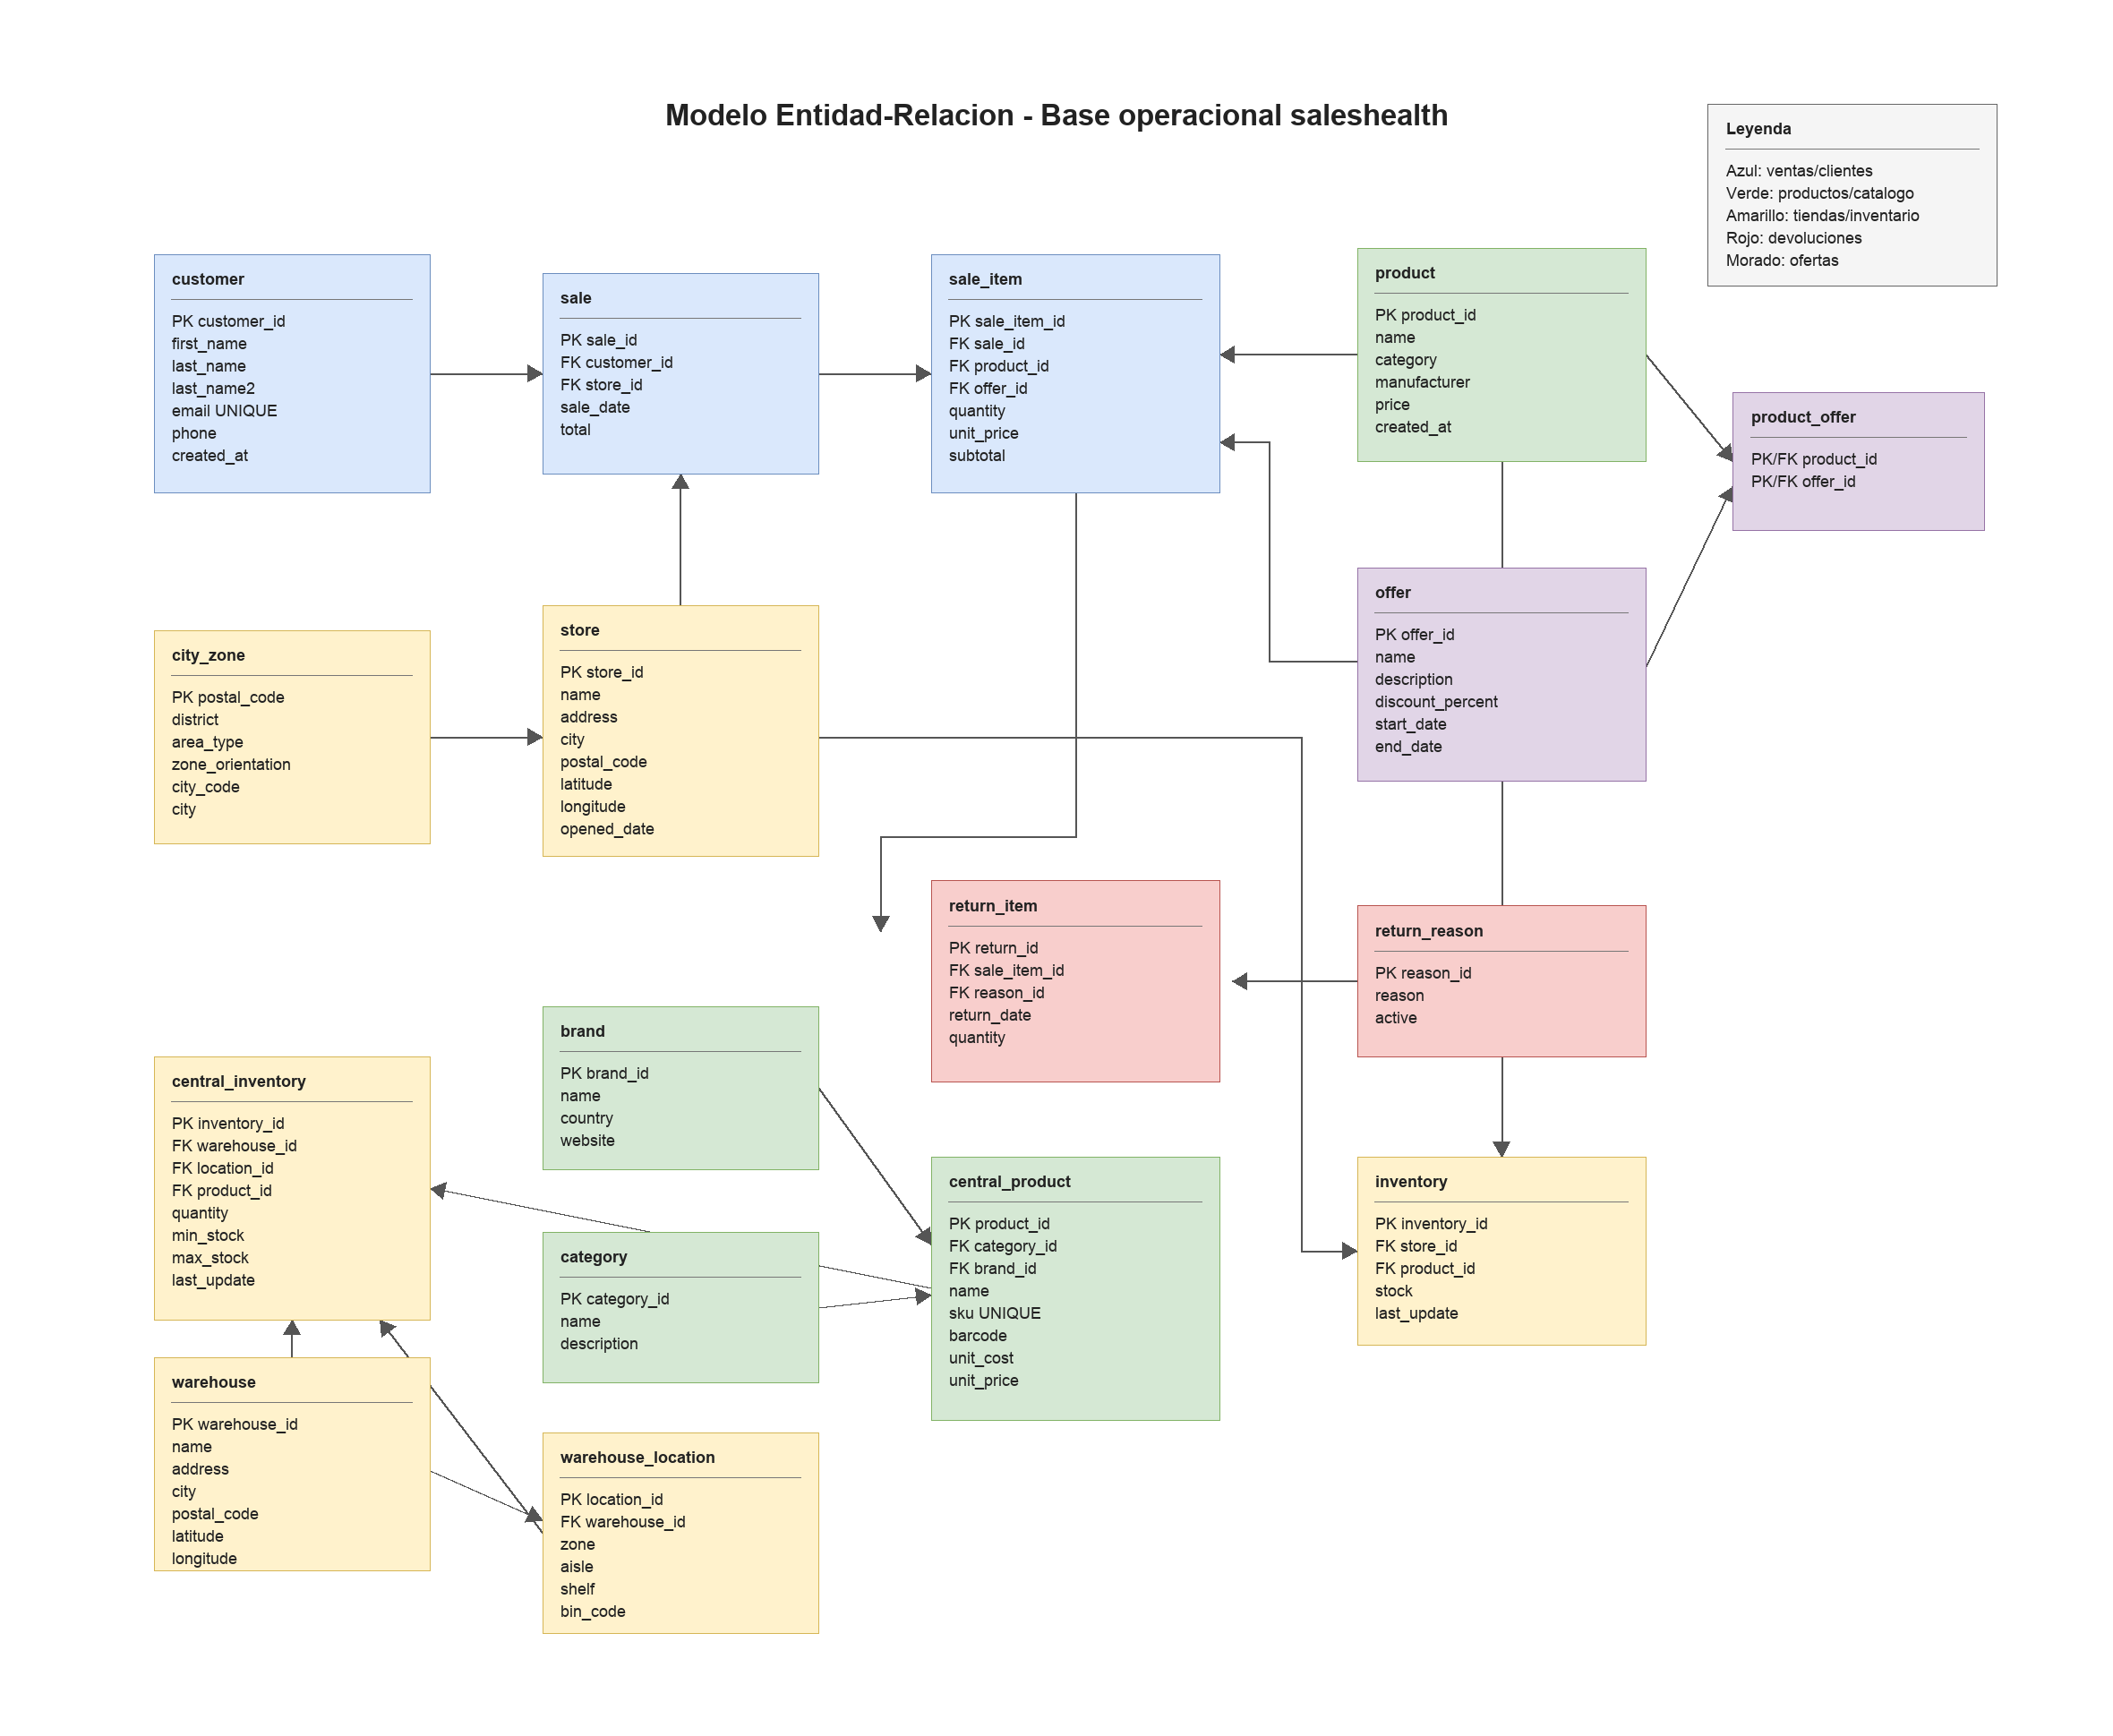
\includegraphics[width=0.68\textwidth,keepaspectratio]{modelo_er_original.png}
\caption{Modelo Entidad-Relación de la base operacional saleshealth
(17 tablas).}
\end{figure}

\subsection{Modelo dimensional --- constelación de hechos}

El esquema \textbf{dwh} implementa cuatro tablas de hechos independientes
que comparten ocho dimensiones comunes. El grano principal es la línea de
venta (\texttt{sale\_item\_id}).

\vspace{3pt}
\begin{tabularx}{\textwidth}{L{3.0cm}X}
\toprule
\Th{Decisión} & \Th{Justificación} \\
\midrule
\Ra Constelación de hechos
  & Ventas, devoluciones e inventario tienen granularidades distintas, pero
    comparten cliente, producto, fecha y localización. \\
\Rb Claves surrogate
  & Aíslan el DWH de cambios en identificadores operacionales y facilitan
    integridad referencial. \\
\Ra Registro técnico
  & «Sin oferta» y «Sin motivo» evitan claves nulas y mantienen cobertura
    completa de hechos. \\
\Rb Coste analítico
  & El coste original se conserva; el coste imputado se marca con
    \texttt{cost\_source} para no ocultar calidad de dato. \\
\bottomrule
\end{tabularx}

\vspace{5pt}
El modelo resultante permite analizar margen y devoluciones con el mismo
grano de venta, valorar inventario por tienda y almacén central, y conectar
las métricas de cliente con productos, tiendas y periodos sin duplicar reglas
de negocio en cada consulta.

\vspace{5pt}
\begin{center}
\begin{tabular}{@{}C{2.6cm}C{2.6cm}C{2.6cm}C{2.6cm}@{}}
\toprule
\Th{Ventas} & \Th{Devol.} & \Th{Inv. tienda} & \Th{Inv. central} \\
\midrule
\Ra Ventas & Devoluciones & Stock tienda & Stock central \\
\Rb Línea venta & Línea devuelta & Stock tienda & Stock almacén \\
\bottomrule
\end{tabular}
\end{center}

%% ── FIGURA DWH (misma página que 2.2) ────────────────────────────────────
\begin{figure}[H]
\centering
% DWH es vertical (2360x3550): height=0.84textheight mantiene todo en una página
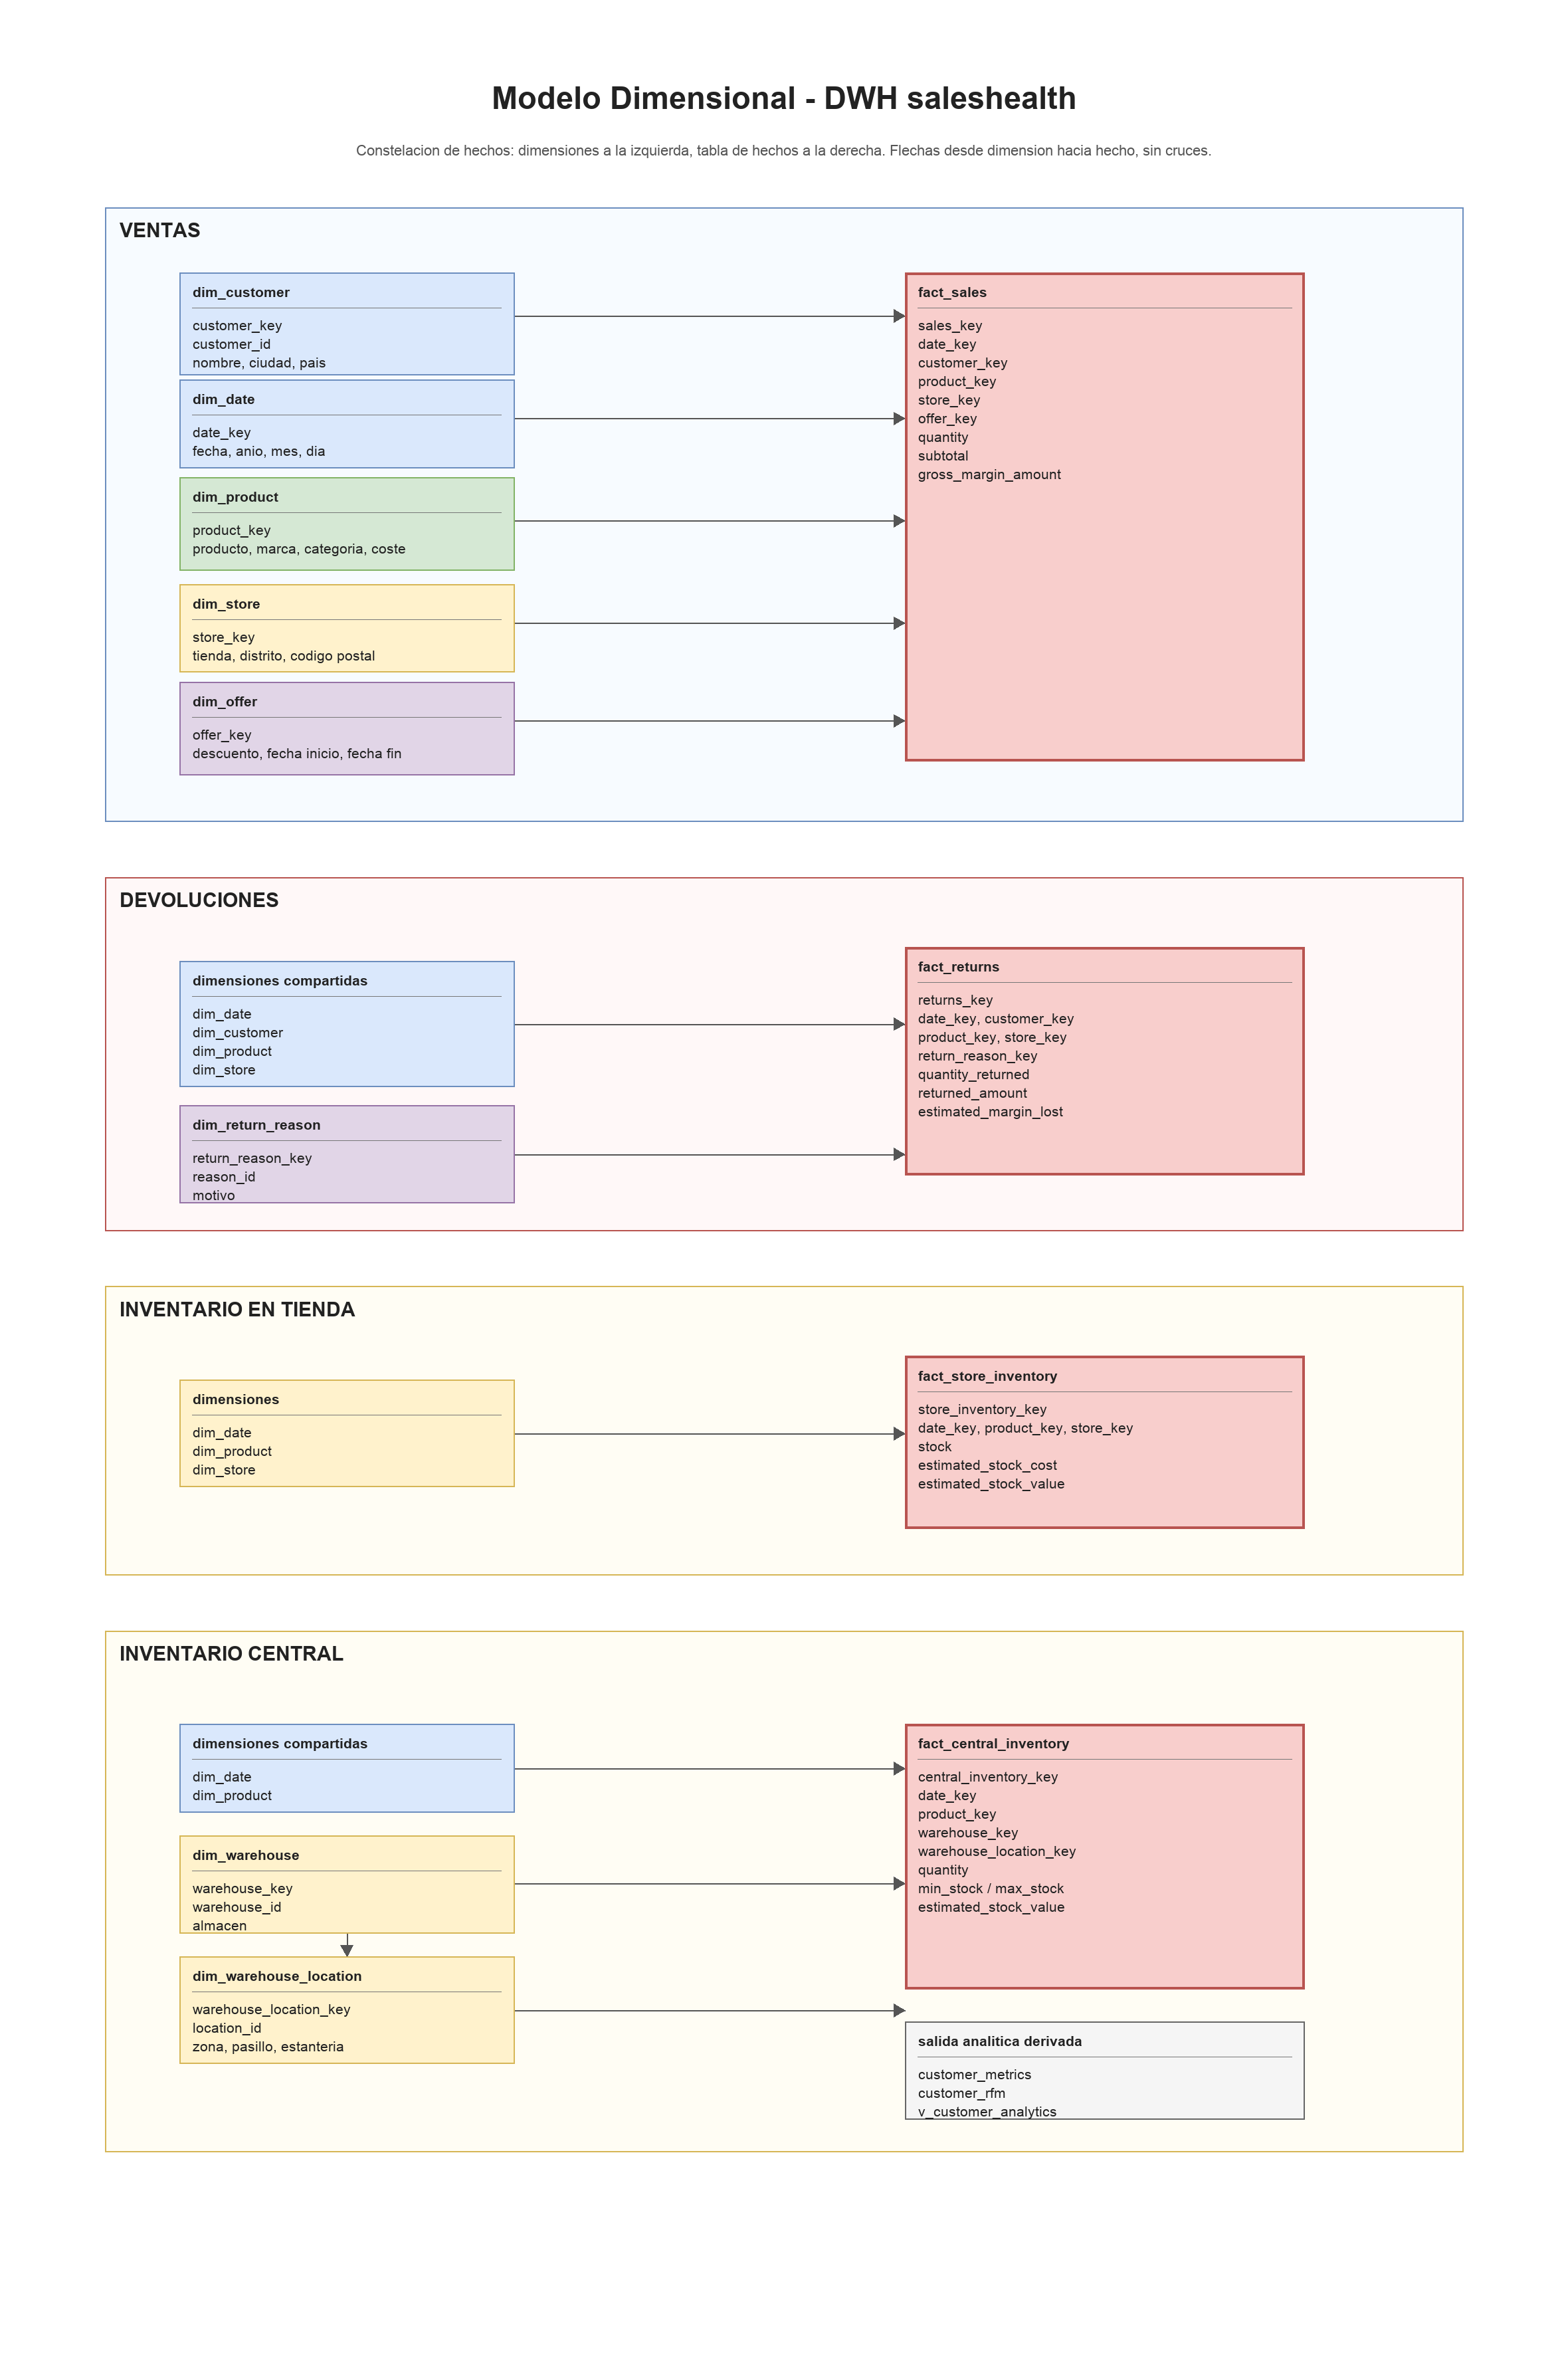
\includegraphics[height=0.42\textheight,keepaspectratio]{modelo_dimensional_dwh.png}
\caption{Modelo dimensional del DWH saleshealth --- constelación de hechos
(ventas, devoluciones, inventario en tienda e inventario central).}
\end{figure}

%% ── PÁGINA 4: ETL + CLTV + RFM ─────────────────────────────
\section{ETL, calidad de margen y métricas de cliente}

\subsection{Proceso ETL}

El ETL (\textit{sql/02\_etl.sql}) carga el DWH en una única transacción
atómica. Incluye generación de calendario via \texttt{generate\_series},
enriquecimiento de tiendas con \texttt{city\_zone}, registros técnicos para
ofertas y motivos ausentes, y cálculo de coste y margen por línea.

La carga es idempotente: puede repetirse sin acumular registros residuales. Esta
propiedad es importante en un entorno académico reproducible, pero también en
un entorno real, porque permite reconstruir el DWH completo cuando cambian las
reglas de transformación o se corrige una incidencia en la fuente.

\vspace{5pt}
\begin{center}
\begin{tabular}{@{}C{1.7cm}C{1.7cm}C{1.7cm}C{1.7cm}C{1.7cm}C{1.7cm}@{}}
\toprule
\Th{1} & \Th{2} & \Th{3} & \Th{4} & \Th{5} & \Th{6} \\
\midrule
\Ra Crear DWH & Cargar hechos & Métricas & Clusters & Basket & Validar \\
\Rb \texttt{01} & \texttt{02} & \texttt{03} & \texttt{05} & \texttt{06} & \texttt{04} \\
\bottomrule
\end{tabular}
\end{center}

\begin{mdframed}[style=cbox]
\textbf{\color{accent}Incidencia producto 29 --- coste imputado trazable}\\[2pt]
El «Sensor temperatura inteligente» aparece en 711 líneas sin coste en
\texttt{central\_product}. El DWH mantiene el coste original nulo y añade
\texttt{analytic\_unit\_cost = sale\_price * 0{,}60}, marcando cada línea con
\texttt{cost\_source = 'IMPUTED\_60\_PCT\_PRICE'} e
\texttt{is\_cost\_imputed = true}. Impacto: 1\,426 unidades, 28\,505\,EUR en
ingresos, 11\,408\,EUR de margen estimado recuperado.
\end{mdframed}

\subsection{CLTV --- tres variantes}

\textbf{CLTV histórico por ingresos}: ingresos netos acumulados por cliente.
\textbf{CLTV histórico por margen}: descuenta el coste estimado; es la métrica
más relevante para priorizar inversión comercial.
\textbf{CLTV estimado a 12 meses}: proyecta el valor esperado según frecuencia
mensual y ticket medio.

La memoria prioriza el CLTV por margen porque el ingreso por sí solo puede
sobrestimar clientes que compran productos de bajo margen o generan muchas
devoluciones. El enfoque por margen permite decidir inversión comercial con
mejor criterio económico.

\subsection{Segmentación RFM}

Cada cliente recibe puntuación 1--5 en Recencia, Frecuencia y Monetario
(\texttt{NTILE(5)}), combinados en seis segmentos:

\vspace{3pt}
\begin{tabularx}{\textwidth}{L{2.9cm}C{1.5cm}L{3.0cm}X}
\toprule
\Th{Segmento} & \Th{Clientes} & \Th{Perfil RFM} & \Th{Acción prioritaria} \\
\midrule
\Ra Clientes estrella  & 1\,218 & Alta R, F y M
  & Fidelización: ventajas exclusivas \\
\Rb Valiosos en riesgo & 726    & Buen valor, baja rec.
  & Recuperación: incentivo limitado \\
\Ra Fieles recientes   & 370    & Alta F, valor mod.
  & Mantenimiento: reforzar hábito \\
\Rb Alto valor         & 356    & Ticket alto, baja F
  & Upselling: mayor margen \\
\Ra Clientes dormidos  & 1\,057 & Baja R y F
  & Reactivación selectiva por margen \\
\Rb Clientes medios    & 2\,023 & Comportamiento medio
  & Campañas genéricas \\
\bottomrule
\end{tabularx}

\vspace{4pt}
Los 1\,218 clientes estrella y los 726 valiosos en riesgo concentran la mayor
parte del margen histórico y justifican inversión comercial prioritaria.
La segmentación traduce métricas técnicas en acciones: fidelizar, reactivar,
mantener o tratar mediante campañas genéricas según valor y recencia.

\vspace{5pt}
\begin{center}
\begin{tabularx}{0.88\textwidth}{L{3.0cm}X}
\toprule
\Th{Criterio} & \Th{Uso en la priorización} \\
\midrule
\Ra Valor alto + recencia alta & Mantener relación y ofrecer venta cruzada. \\
\Rb Valor alto + recencia baja & Reactivar antes de que el cliente desaparezca. \\
\Ra Valor bajo + riesgo alto & Automatizar seguimiento, sin inversión intensiva. \\
\bottomrule
\end{tabularx}
\end{center}

%% ── PÁGINA 5: CHURN + CLUSTERING ───────────────────────────
\section{Scoring de churn y segmentación por clustering}

\subsection{Scoring de churn}

El scoring combina cuatro señales en un índice de 0 a 100: \textbf{recencia},
\textbf{frecuencia mensual}, \textbf{tasa de devolución} y \textbf{valor
histórico por margen}.

No se presenta como un modelo predictivo supervisado, sino como un score
heurístico de priorización. Su ventaja es la explicabilidad: cada cliente puede
ordenarse por riesgo y cada acción recomendada se entiende a partir de variables
observables del DWH.

\vspace{3pt}
\begin{tabularx}{\textwidth}{L{1.7cm}C{1.7cm}L{4.3cm}X}
\toprule
\Th{Nivel} & \Th{Score} & \Th{Lectura} & \Th{Acción recomendada} \\
\midrule
\Ra Bajo    & 0--25   & Cliente activo y recurrente
  & Seguimiento normal \\
\Rb Medio   & 26--50  & Señales de distanciamiento
  & Atención comercial proactiva \\
\Ra Alto    & 51--75  & Caída visible de actividad
  & Campaña de reactivación \\
\Rb Crítico & 76--100 & Riesgo inminente de abandono
  & Recuperación prioritaria \\
\bottomrule
\end{tabularx}

\vspace{4pt}
Los 5\,750 clientes tienen score, nivel y acción recomendada asignados,
permitiendo ordenar la cartera completa por riesgo de forma objetiva.
El score se usa como complemento de CLTV: un cliente de alto valor y alto
riesgo debe priorizarse antes que un cliente de bajo margen con el mismo nivel
de churn.

\vspace{5pt}
\begin{center}
\begin{tabular}{@{}C{2.6cm}C{2.6cm}C{2.6cm}C{2.6cm}@{}}
\toprule
\Th{Recencia} & \Th{Frecuencia} & \Th{Devoluciones} & \Th{Margen} \\
\midrule
\Ra Distancia desde última compra & Ritmo mensual de compra
& Fricción o insatisfacción & Valor económico histórico \\
\bottomrule
\end{tabular}
\end{center}

\subsection{PCA y clustering K-Means}

PCA sobre las métricas de cliente reduce la dimensionalidad a dos componentes
que explican el 72{,}75\,\% de la variabilidad. K-Means con $k = 4$:

Las variables de entrada combinan comportamiento económico, frecuencia,
recencia y devoluciones. El PCA se utiliza para visualizar patrones, mientras
que la asignación de cluster se almacena en \texttt{dwh.customer\_clusters}
para integrarla después en \texttt{customer\_360}.

\begin{figure}[H]
\centering
\includegraphics[width=0.50\textwidth,keepaspectratio]{clientes_pca_clusters.png}
\caption{Proyección de los 5\,750 clientes sobre PC1/PC2,
coloreados por cluster ($k = 4$).}
\end{figure}

\vspace{-2pt}
{\small
\begin{tabularx}{\textwidth}{C{1.3cm}L{3.3cm}C{1.5cm}C{1.9cm}X}
\toprule
\Th{Cluster} & \Th{Perfil} & \Th{Clientes} & \Th{Churn medio}
  & \Th{Lectura de negocio} \\
\midrule
\Ra 0 & Recientes con potencial & 1\,469 & 20{,}51
  & Candidatos para venta cruzada \\
\Rb 1 & Alto valor              & 746    & 32{,}10
  & Principal fuente de margen \\
\Ra 2 & Inactivos / en riesgo   & 3\,134 & 62{,}72
  & Requieren reactivación selectiva \\
\Rb 3 & Más devoluciones        & 401    & 67{,}59
  & Revisar experiencia y política \\
\bottomrule
\end{tabularx}}

\begin{mdframed}[style=cbox]
\textbf{\color{accent}RFM y clustering son complementarios}\\[2pt]
RFM segmenta con reglas claras. El clustering detecta agrupaciones por
similitud matemática que los quintiles RFM no capturan --- en particular
el cluster 3, con devoluciones extremas, que puede aparecer como «medio»
en RFM pero requiere intervención específica.
\end{mdframed}

%% ── PÁGINA 6: MARKET BASKET ─────────────────────────────────
\section{Market Basket Analysis}

\textit{sql/06\_market\_basket.sql} trata cada ticket como una cesta y
calcula tres métricas para todos los pares de productos:

\vspace{3pt}
\begin{tabularx}{\textwidth}{L{2.1cm}L{5.2cm}X}
\toprule
\Th{Métrica} & \Th{Definición} & \Th{Para qué sirve} \\
\midrule
\Ra Support    & Proporción de tickets con el par
  & Frecuencia de la combinación en el negocio \\
\Rb Confidence & $P(B|A)$ --- prob. de comprar B dado A
  & Base para recomendaciones A $\to$ B \\
\Ra Lift       & Ratio sobre compra esperada por azar
  & Lift $>$ 1 indica asociación real \\
\bottomrule
\end{tabularx}

\vspace{6pt}
Con umbral mínimo de 10 tickets y lift $> 1$ se obtienen \textbf{207 reglas
significativas} y \textbf{235 recomendaciones direccionales}. El lift máximo
es 1{,}3921 --- esos pares se compran un 39\,\% más de lo esperado.

El umbral mínimo evita recomendar asociaciones anecdóticas. Además, se separa
la afinidad bidireccional del par de la recomendación direccional A $\to$ B:
un par puede ser frecuente, pero la recomendación comercial depende de la
probabilidad condicional desde el producto base.

\vspace{4pt}
\begin{tabularx}{\textwidth}{L{5.2cm}C{1.8cm}X}
\toprule
\Th{Indicador} & \Th{Valor} & \Th{Interpretación} \\
\midrule
\Ra Pares producto-producto           & 1\,225
  & Todas las combinaciones entre 50 productos \\
\Rb Recomendaciones direccionales     & 235
  & Pares A $\to$ B donde lift $> 1$ \\
\Ra Reglas con lift $>1$ y 10+ tickets& 207
  & Con soporte mínimo y asociación demostrada \\
\Rb Lift máximo                       & 1{,}3921
  & Mayor fuerza de asociación observada \\
\bottomrule
\end{tabularx}

\begin{mdframed}[style=cbox]
\textbf{\color{accent}Tres aplicaciones comerciales inmediatas}\\[2pt]
\textbf{Packs de producto:} combinar pares con mayor lift y revenue medio
en una oferta específica.
\textbf{Cross-selling en ficha:} «los clientes que compran X también
compran Y».
\textbf{Promociones cruzadas:} descuentos condicionados a compra conjunta
de los pares más frecuentes. Todas las decisiones tienen respaldo estadístico.
\end{mdframed}



\vspace{5pt}
\begin{center}
\begin{tabular}{@{}C{2.4cm}C{2.4cm}C{2.4cm}C{2.4cm}@{}}
\toprule
\Th{Ticket} & \Th{Pares} & \Th{Métricas} & \Th{Recom.} \\
\midrule
\Ra Ticket & Producto A + B & Support, confidence, lift
& Producto base $\to$ sugerido \\
\bottomrule
\end{tabular}
\end{center}

%% ── PÁGINA 7: CUSTOMER 360 ──────────────────────────────────
\section{Customer 360}

El mart \texttt{dwh.customer\_360} consolida en una única vista, con una
fila por cliente, todo lo calculado en el proyecto:

\vspace{3pt}
\begin{tabularx}{\textwidth}{L{2.6cm}X}
\toprule
\Th{Bloque} & \Th{Información incluida} \\
\midrule
\Ra Identificación & \texttt{customer\_id}, nombre, email, fecha de alta \\
\Rb Actividad      & Primera y última compra $\cdot$ compras $\cdot$
  recencia $\cdot$ frecuencia \\
\Ra Económica      & Ingresos brutos y netos $\cdot$ margen $\cdot$
  ticket medio $\cdot$ importe devuelto \\
\Rb CLTV           & Histórico por ingresos $\cdot$ histórico por margen
  $\cdot$ estimado a 12 meses \\
\Ra Riesgo         & \texttt{churn\_risk\_score} $\cdot$
  \texttt{churn\_risk\_level} $\cdot$ \texttt{recommended\_action} \\
\Rb Clustering     & \texttt{cluster\_id} $\cdot$ \texttt{cluster\_name}
  $\cdot$ coordenadas PCA $\cdot$ distancia al centroide \\
\bottomrule
\end{tabularx}

\vspace{6pt}
Esta integración es el valor diferencial: no se trata de tener métricas por
separado, sino en una única entidad consultable que el dashboard expone,
las validaciones protegen y el diccionario documenta.

Cada fila de \texttt{customer\_360} funciona como una ficha analítica de
cliente. Integra valor, frecuencia, recencia, devoluciones, churn, RFM y cluster
para que una consulta comercial no dependa de unir manualmente seis tablas
intermedias.

\begin{mdframed}[style=cbox]
\textbf{\color{accent}Por qué \texttt{customer\_360} cambia la forma de trabajar}\\[2pt]
Antes de este proyecto, responder «¿cuáles son mis 50 clientes más valiosos
en riesgo de abandono?» requería cruzar manualmente varias tablas. Con
\texttt{customer\_360} la consulta es directa: ordenar por CLTV por margen
descendente y filtrar por
\texttt{churn\_risk\_level = 'Crítico'} o \texttt{'Alto'}.
El resultado incluye nombre, segmento RFM, cluster y acción recomendada
en una sola fila --- sin intermediarios.
\end{mdframed}

\vspace{3pt}
Este mart también simplifica el dashboard: las páginas de segmentación, churn y
cliente individual consumen una misma capa semántica. Así se reduce el riesgo
de que dos visualizaciones calculen la misma métrica de forma diferente.

\vspace{5pt}
\begin{center}
\MiniBox{2.0cm}{Identidad\\cliente}
\hspace{4pt}
\MiniBox{2.0cm}{Actividad\\compras}
\hspace{4pt}
\MiniBox{2.0cm}{Valor\\CLTV}
\hspace{4pt}
\MiniBox{2.0cm}{Riesgo\\churn}
\hspace{4pt}
\MiniBox{2.0cm}{Perfil\\cluster}
\end{center}

%% ── PÁGINA 8: VALIDACIONES + DASHBOARD ─────────────────────
\section{Validaciones y dashboard ejecutivo}

\subsection{Validaciones reproducibles --- 14/14 OK}

\textit{sql/04\_validaciones\_dwh.sql} ejecuta 14 controles automáticos
al final de cada ejecución del pipeline:

\vspace{3pt}
\begin{tabularx}{\textwidth}{L{3.0cm}L{8.0cm}C{1.7cm}}
\toprule
\Th{Categoría} & \Th{Controles} & \Th{OK} \\
\midrule
\Ra Integridad    & Volumen de cada tabla coincide con la fuente $\cdot$
  Claves dimensionales no nulas & 6/6 OK \\
\Rb Cobertura     & Métricas para todos $\cdot$ Churn score $\cdot$
  Clusters $\cdot$ RFM $\cdot$ \texttt{customer\_360} completo & 5/5 OK \\
\Ra Calidad datos & Reglas MBA presentes $\cdot$ Recomendaciones generadas
  $\cdot$ Coste imputado trazado & 3/3 OK \\
\bottomrule
\end{tabularx}

\vspace{4pt}
El resultado \textbf{14/14 OK} certifica que el DWH es consistente con la
fuente y que todas las capas analíticas tienen cobertura total sobre los
5\,750 clientes.

Las validaciones cubren tres niveles: integridad entre origen y hechos,
cobertura de métricas analíticas y control específico de la incidencia del
producto 29. Esto convierte la calidad de datos en una fase automatizada, no
en una revisión manual posterior.

\newgeometry{
  top=3.0cm, bottom=0.45cm,
  left=1.9cm, right=1.9cm,
  headheight=14pt
}
\newpage
\vspace*{1.0cm}
\subsection{Dashboard ejecutivo Saleshealth}

Implementado en Streamlit con Plotly, alimentado por tres CSV versionados
que permiten ejecutarlo sin conexión a la base de datos.

La decisión de usar CSVs versionados no sustituye al DWH: permite desplegar una
demo estable y portable. El origen de verdad sigue siendo PostgreSQL, pero el
dashboard puede presentarse sin depender de credenciales ni disponibilidad del
servidor local.

\vspace{5pt}
\begin{center}
\begin{tabularx}{0.88\textwidth}{L{3.0cm}X}
\toprule
\Th{Artefacto} & \Th{Rol en la demo} \\
\midrule
\Ra Customer analytics & Métricas de cliente, RFM y churn. \\
\Rb Customer clusters & Coordenadas PCA y perfil de cluster. \\
\Ra Product recs. & Reglas de recomendación producto-producto. \\
\bottomrule
\end{tabularx}
\end{center}

\vspace{3pt}
\begin{tabularx}{\textwidth}{L{3.4cm}X}
\toprule
\Th{Página} & \Th{Contenido} \\
\midrule
\Ra 1. Resumen ejecutivo & KPIs globales, margen por segmento RFM,
  distribución de churn \\
\Rb 2. Customer 360      & Buscador por cliente, ficha completa con CLTV,
  RFM, churn, cluster y acción \\
\Ra 3. Segmentación      & Distribución RFM y por cluster, scatter PCA
  interactivo \\
\Rb 4. Churn             & Clientes Alto/Crítico, churn medio por segmento,
  top en riesgo \\
\Ra 5. Market Basket     & Filtro por producto, top recomendaciones por lift,
  glosario \\
\Rb 6. Calidad de datos  & Caso producto 29 cuantificado,
  tabla 14/14 validaciones \\
\bottomrule
\end{tabularx}

\vspace{5pt}
\textbf{Reproducibilidad.} El proyecto se ejecuta con
\texttt{scripts/run\_pipeline.sh}, que lanza la creación del DWH, ETL,
métricas, carga de clusters, Market Basket y validaciones. Los notebooks
\texttt{00}--\texttt{06} documentan la exploración y los CSV versionados
permiten abrir el dashboard sin depender de una conexión activa a PostgreSQL.

\vspace{6pt}
\begin{tabularx}{\textwidth}{C{1.2cm}L{3.5cm}X}
\Th{No.} & \Th{Script} & \Th{Función en el pipeline} \\
\Ra 0 & Explorar origen
  & Exploración inicial del origen: conteos, relaciones y calidad. \\
\Rb 1 & Crear DWH
  & Crea dimensiones, hechos, tablas analíticas y vistas del esquema
    \texttt{dwh}. \\
\Ra 2 & ETL
  & Carga dimensiones y hechos desde saleshealth, calcula coste y margen. \\
\Rb 3 & Métricas CLTV
  & Construye métricas de cliente, CLTV, RFM, churn y
    \texttt{customer\_360}. \\
\Ra 4 & Clustering Python
  & Genera PCA y K-Means desde \texttt{customer\_analytics.csv}. \\
\Rb 5 & Cargar clusters
  & Carga clusters en PostgreSQL y los integra con cliente. \\
\Ra 6 & Market Basket
  & Calcula afinidad producto-producto y recomendaciones comerciales. \\
\Rb 7 & Validaciones
  & Ejecuta 14 controles automáticos de integridad, cobertura y calidad. \\
\end{tabularx}

\vspace{6pt}
\begin{center}\scriptsize
\begin{tabular}{@{}C{1.25cm}C{1.25cm}C{1.25cm}C{1.25cm}C{1.25cm}C{1.25cm}C{1.25cm}@{}}
\Th{00} & \Th{01} & \Th{02} & \Th{03} & \Th{04} & \Th{05} & \Th{06} \\
\Ra Conex. & Invent. & Relac. & EDA & Cliente & Cluster & Basket \\
\end{tabular}
\end{center}

\vspace{2pt}
Los archivos exactos ejecutados son los siete SQL de la carpeta sql
(00 exploración, 01 DWH, 02 ETL, 03 métricas, 05 carga de clusters,
06 Market Basket y 04 validaciones), más el script Python de clustering
para generar PCA y K-Means.

\vspace{3pt}
El pipeline de notebooks sigue la misma lógica que el DWH: primero verifica
conexión y estructura, después identifica relaciones implícitas y problemas de
calidad, continúa con EDA de negocio, y finalmente desarrolla las capas
analíticas de cliente, clustering y Market Basket. El notebook
\texttt{analisis\_clientes.ipynb} queda como resumen ejecutivo final sin
duplicar todo el desarrollo metodológico.

\newpage
\vspace*{1.0cm}

%% ── ÚLTIMA PÁGINA: CONCLUSIONES + LIMITACIONES ─────────────
\section{Conclusiones y acciones recomendadas}

La conclusión principal: \textbf{no todos los clientes deben tratarse igual}.
RFM, clustering y churn permiten ordenar la cartera por valor y riesgo, y
proponer acciones diferenciadas con base cuantitativa. La prioridad no se
asigna por intuición, sino por margen histórico, recencia, churn y patrón de
compra.

\vspace{-2pt}
\begin{tabularx}{\textwidth}{L{2.9cm}C{0.8cm}X C{1.45cm}}
\toprule
\Th{Segmento} & \Th{N} & \Th{Acción recomendada} & \Th{Nivel} \\
\midrule
\Ra Clientes estrella  & 1\,218 & Fidelización personalizada & Alta \\
\Rb Valiosos en riesgo & 726    & Reactivación con incentivo y revisión de devoluciones & Alta \\
\Ra Fieles recientes   & 370    & Mantener hábito de compra & Media \\
\Rb Alto valor         & 356    & Upselling y productos de mayor margen & Media \\
\Ra Clientes dormidos  & 1\,057 & Reactivación selectiva por margen histórico & Selectiva \\
\Rb Clientes medios    & 2\,023 & Campañas genéricas & Baja \\
\bottomrule
\end{tabularx}

\vspace{3pt}
\begin{mdframed}[style=cbox]
\textbf{\color{accent}Lectura final}\\[2pt]
El modelo dimensional mejora la consulta; CLTV/RFM/churn convierten ventas en
conocimiento de cliente; el clustering descubre perfiles no evidentes; y
Market Basket transforma tickets históricos en recomendaciones accionables.
\end{mdframed}

\vspace{2pt}
\begin{center}
\begin{tabular}{@{}C{3.1cm}C{3.1cm}C{3.1cm}@{}}
\toprule
\Th{Proteger} & \Th{Recuperar} & \Th{Optimizar} \\
\midrule
\Ra Clientes estrella y alto valor
& Valiosos en riesgo y dormidos rentables
& Devoluciones y packs por afinidad \\
\bottomrule
\end{tabular}
\end{center}

\section{Limitaciones, mejoras futuras y cierre}

\begin{tabularx}{\textwidth}{L{3.0cm}X}
\toprule
\Th{Área} & \Th{Limitación y mejora propuesta} \\
\midrule
\Ra CLTV & La proyección a 12 meses asume continuidad histórica; mejora natural:
modelos BG/NBD + Gamma-Gamma. \\
\Rb Clustering & K-Means depende de variables, escalado y $k$; se puede refinar
con codo y silhouette. \\
\Ra Calidad origen & El producto 29 requiere corregir el coste real en el catálogo
central. \\
\Rb Evolución & Añadir series temporales mensuales de ingresos, margen y
devoluciones. \\
\Ra Infraestructura & Evolucionar a dbt/Airflow y validaciones tipo Great
Expectations. \\
\bottomrule
\end{tabularx}

\vspace{3pt}
\begin{mdframed}[style=cbox]
\textbf{\color{accent}Cierre del proyecto}\\[2pt]
El proyecto demuestra el ciclo completo de gestión de datos: origen, DWH, ETL,
métricas, clustering, Market Basket, validación y dashboard. La aportación
diferencial es \texttt{customer\_360}: una fila por cliente con valor, riesgo,
segmento, cluster y acción comercial recomendada.
\end{mdframed}

\vspace{3pt}
\begin{center}
\small\itshape\color{mutedgray}
17 tablas $\cdot$ 8 dimensiones $\cdot$ 4 hechos $\cdot$ 5\,750 clientes
con CLTV/RFM/churn/cluster $\cdot$ 1\,225 pares $\cdot$ 235 recomendaciones
$\cdot$ 14/14 validaciones OK $\cdot$ dashboard de 6 páginas.
\end{center}

\end{document}
